%%% Template originaly created by Karol Kozioł (mail@karol-koziol.net) and modified for ShareLaTeX use

\documentclass[a4paper,11pt]{article}

\usepackage[T1]{fontenc}
\usepackage[utf8]{inputenc}
\usepackage{graphicx}
\usepackage{xcolor}

\renewcommand\familydefault{\sfdefault}
\usepackage{tgheros}
\usepackage[defaultmono]{droidmono}

\usepackage{amsmath,amssymb,amsthm,textcomp}
\usepackage{enumerate}
\usepackage{multicol}
\usepackage{tikz}

\usepackage{geometry}
\geometry{total={210mm,297mm},
left=25mm,right=25mm,%
bindingoffset=0mm, top=20mm,bottom=20mm}


\linespread{1.3}

\newcommand{\linia}{\rule{\linewidth}{0.5pt}}

% custom theorems if needed
\newtheoremstyle{mytheor}
    {1ex}{1ex}{\normalfont}{0pt}{\scshape}{.}{1ex}
    {{\thmname{#1 }}{\thmnumber{#2}}{\thmnote{ (#3)}}}

\theoremstyle{mytheor}
\newtheorem{defi}{Definition}

% my own titles
\makeatletter
\renewcommand{\maketitle}{
\begin{center}
\vspace{2ex}
{\huge \textsc{\@title}}
\vspace{1ex}
\\
\linia\\
\@author \hfill \@date
\vspace{4ex}
\end{center}
}
\makeatother
%%%

% custom footers and headers
\usepackage{fancyhdr}
\pagestyle{fancy}
\lhead{}
\chead{}
\rhead{}
\lfoot{PI : Rubik's Cube}
\cfoot{}
\rfoot{Page \thepage}
\renewcommand{\headrulewidth}{0pt}
\renewcommand{\footrulewidth}{0pt}
%
\usepackage{hyperref}
% code listing settings
\usepackage{listings}
\lstset{
    language=Java,
    basicstyle=\ttfamily\small,
    aboveskip={1.0\baselineskip},
    belowskip={1.0\baselineskip},
    columns=fixed,
    extendedchars=true,
    breaklines=true,
    tabsize=4,
    prebreak=\raisebox{0ex}[0ex][0ex]{\ensuremath{\hookleftarrow}},
    frame=lines,
    showtabs=false,
    showspaces=false,
    showstringspaces=false,
    keywordstyle=\color[rgb]{0.627,0.126,0.941},
    commentstyle=\color[rgb]{0.133,0.545,0.133},
    stringstyle=\color[rgb]{01,0,0},
    numbers=left,
    numberstyle=\small,
    stepnumber=1,
    numbersep=10pt,
    captionpos=t,
    escapeinside={\%*}{*)}
}

%%%----------%%%----------%%%----------%%%----------%%%

\begin{document}

\title{Projet Informatique : Résoudre de façon optimale le Rubik's Cube.}

\author{Achari Berrada Youssef, Boumahdi Réda}

\date{12/01/2015}

\maketitle



\section*{Introduction :}
Malgré le fait que le projet est difficile, nous avons choisi le PI Rubik's Cube car nous avons voulu découvrir comment fonctionne ce casse tête qui nous a si longuement occupé pendant notre jeune âge et nous a fasciné autant par la simplicité de l'enjeu que par la difficulté de le réaliser.

Notre projet informatique formé par le code ainsi que par le présent rapport, est présent sur le lien du github suivant : \underline{\href{https://github.com/YabTag/RubiksCube}{github.com/YabTag/RubiksCube}}. Nous avons choisi d'utiliser cet outil pour des raisons pratiques évidentes.

\section{Configuration :}

\subsection{Représentation du Rubik's Cube : }

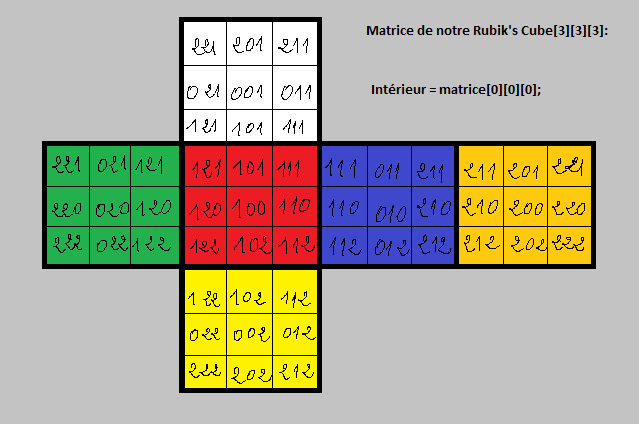
\includegraphics[scale=1]{RubiksCube.png}

Nous avons choisi de représenter notre cube sous la forme d'une matrice à trois dimensions. Tout d'abord, on suppose que notre cube est fixe, si bien que parler de haut du cube n'est pas ambigu, il s'agit de la face du haut. Ensuite, chaque élément de la matrice contient un objet du type « Piece », cet objet est un tableau à 6 éléments, dans l'ordre suivant « haut, bas, gauche, droite, derrière, en face » initialisé à -1. Nous représentons les couleurs comme étant des entiers de 0 à 5. Ainsi pour représenter une pièce donnée, on utilise le fait qu'elle partage une couleur avec différentes faces. Aussi, si on parle de la pièce qui partage une couleur avec la face gauche et la face haut, il n'y a pas d'ambiguïté, il n'y en a qu'une seule : les 2 autres sont des sommets, et aussi elles partagent nécessairement une troisième couleur avec une autre face. Pour se repérer entre les faces, il s'agit de remarquer qu'en réalité, le centre de chaque face est fixe, du coup la face est repérable par la couleur du centre de chaque face. Enfin, les pièces étant numérotées de façon bijective, nous savons toujours à quel moment quelle pièce représente le centre haut gauche de la face gauche par exemple.


\begin{lstlisting}[label={list:first},caption=La classe du notre Rubik's cube.]
public class Rubiks {
	
	public Piece[][][] matrice = new Piece[3][3][3];
	
	public void setRubiks(){
		//Interieur*1
		matrice[0][0][0]= new Piece(-1,-1,-1,-1,-1,-1);
		//6 Centres qui restent invariables
		matrice[1][0][0]= new Piece(0,-1,-1,-1,-1,-1);
		matrice[2][0][0]= new Piece(-1,1,-1,-1,-1,-1);
		matrice[0][1][0]= new Piece(-1,-1,2,-1,-1,-1);
		matrice[0][2][0]= new Piece(-1,-1,-1,3,-1,-1);
		matrice[0][0][1]= new Piece(-1,-1,-1,-1,4,-1);
		matrice[0][0][2]= new Piece(-1,-1,-1,-1,-1,5);
		// Arete * 12
		matrice[1][1][0]= new Piece(0,-1,2,-1,-1,-1);
		matrice[1][2][0]= new Piece(0,-1,-1,3,-1,-1);
		matrice[2][1][0]= new Piece(-1,1,2,-1,-1,-1);
		matrice[2][2][0]= new Piece(-1,1,-1,3,-1,-1);
		matrice[0][1][1]= new Piece(-1,-1,2,-1,4,-1);
		matrice[0][1][2]= new Piece(-1,-1,2,-1,-1,5);
		matrice[0][2][1]= new Piece(-1,-1,-1,3,4,-1);
		matrice[0][2][2]= new Piece(-1,-1,-1,3,-1,5);
		matrice[1][0][1]= new Piece(0,-1,-1,-1,4,-1);
		matrice[1][0][2]= new Piece(0,-1,-1,-1,-1,5);
		matrice[2][0][1]= new Piece(-1,1,-1,-1,4,-1);
		matrice[2][0][2]= new Piece(-1,1,-1,-1,-1,5);
		// Coin * 8
		matrice[1][1][1]= new Piece(0,-1,2,-1,4,-1);
		matrice[1][1][2]= new Piece(0,-1,2,-1,-1,5);
		matrice[1][2][1]= new Piece(0,-1,-1,3,4,-1);
		matrice[1][2][2]= new Piece(0,-1,-1,3,-1,5);
		matrice[2][1][1]= new Piece(-1,1,2,-1,4,-1);
		matrice[2][1][2]= new Piece(-1,1,2,-1,-1,5);
		matrice[2][2][1]= new Piece(-1,1,-1,3,4,-1);
		matrice[2][2][2]= new Piece(-1,1,-1,3,-1,5);
	}
	public Rubiks(){
		setRubiks();
	}
}	
\end{lstlisting}

Par conséquent, cette représentation permet à tout moment de repérer chaque pièce de notre Rubik's cube et de donner un sens à quelle pièce partage quelle couleur avec quelle face, c'est donc une représentation plausible.


\subsection{Premières fonctions}

Avec notre représentation, remplir et afficher un texte revient à déterminer dans un premier temps la couleur du centre, pour savoir de quelle face il s'agit, ensuite de déterminer quelle couleur est partagée par quelle face. Cette opération se traduit par le parcours de chaque matrice, si on considére la forme développée du cube comme dans la figure 3 de l'énoncé, on suppose que l'on a comme entrée une liste de 6 matrices correspondants dans un ordre donné à celles que l'on voit. Dans ce cas, on parcourt chaque matrice, et on remplit les pièces comme on les voit, il faut en revanche remarquer qu'il faut revenir sur certaines pièces à remplir deux fois ou trois fois. 
\\
L'affiche en revanche est plus simple, il s'agit d'afficher chaque face, en commençant par gauche, jusqu'à la droit. Nous repérons la face gauche comme étant le troisième élément dans le tableau de la pièce, et ainsi de suite pour chaque pièce, dans l'ordre puisque nous savons où est chaque pièce grâce à sa numérotation dans la matrice 3 x 3 x 3.
\\
Enfin, se pose la question de pouvoir permuter les différentes faces de notre Rubik's cube. Ainsi, on prend en compte la face à tourner, en attribuant à la face la couleur de son centre, on sait de quelle face il s'agit. Ensuite, il s'agit de savoir si c'est un quart de tour ou un demi tour, qui est aussi un argument pris par la fonction. A partir de là, il s'agit de faire la permutation des couleurs correpondantes. En réalité, il suffit juste de permuter les couleurs de la pièce en cours avec la pièce correspondante, pour cela, on retrouve dans la matrice les 2 pièces dont on échange les couleurs.


%\begin{lstlisting}[label={list:second},caption=Sample Bash code.]

%\end{lstlisting}

\section{Recherche d'une Solution Optimale :}

\subsection{Un peu de combinatoire :}
Le cube contient 8 sommets qui peuvent être permutés entre eux, et chaque sommet a 3 états possibles. Seulement, l'état du $8^{ième}$ sommet est déterminé par les 7 autres. Ainsi, il y a $8 ! * 3⁷$ configurations différentes pour les sommets.

De plus, le cube contient $12$ arrêtes, les arrêtes étant interchangeables, et ayant 2 états possibles cela donnerait un facteur $12 ! * 2¹²$. Or, encore une fois, l'état de la $12^{ième}$ arrête est déterminé par les 11 autres, et donc en réalité il existe seulement $12 ! * 2¹¹$ configurations différentes.
Enfin, lorsque tous les petites pièces sont bien positionnées, on ne peut permuter 2 pièces sans changer 2 autres pièces entre elles. Cette contrainte supplémentaire diminue le nombre de possibilités par 2.

Finalement, le nombre de possibilité est en fait : $8 ! * 3⁷ * 12 ! * 2¹⁰ = 43252003274489856000.$

Nous remarquons qu'il y a une erreur dans l'énoncé sur ce fait, effectivement, si le résultat $43252003274489856000$ est correct, et cela a été retrouvé dans la documentation, le logiciel Scilab
a permis de lever l'indétermination, des deux formules, c'est $8 ! * 3⁷ * 12 ! * 2¹⁰$ qui donne ce
résultat.


\subsection{L'algorithme IDA : }
Le but de la combinatoire précédante était de nous dissuader de visiter tous les neouds de notre graphe, donc en réalité, nous adaptons notre algorithme pour des cubes peu mélangés. A partir d'un état donné, nous ne visitons que des profondeurs fixés. On visite différents noeuds tout en prenant soin de ne retenir que le chemin courant, et à chaque noeud, on a donc 18 chemins possibles différents, donc des choix différents. Récursivement, si on décide de suivre un chemin donné, et qu'il revient sur un autre élément que nous avons déjà visité, c'est que c'est un cycle, et donc on l'abandonne, et donc on revient un cran en arrière et on en visite un autre, si ils sont tous visités, on revient deux cran en arrière, etc, sinon on poursuit notre exploration jusqu'à atteindre la taille de $l$ éléments. Cependant, la complexité est très grande, dans la mesure où on visite de nombreux noeuds et à chaque rang, on compare le noeud courant aux noeuds gardés en mémoire, en effet, dès qu'on mélange le cube à plus de 5 opérations, l'ordinateur met trop de temps à trouver le bon chemin, mais pour autant on sauve la complexité en mémoire.

\\
Une idée pour ne pas avoir à visiter trop de noeuds suggérer par l'énoncé est d'avoir une fonction renvoyant le nombre minimal d'opérations à effectuer. Effectivement, c'est bien un minorant dont nous avons besoin, car cela nous permettrait d'abandonner un chemin dès que celui ci va trop loin. Si deux chemins différents nous permettent d'aller d'un sommet $s$ vers un sommet $t$, c'est la taille du plus petit chemin qui nous intéresse pour nous arrêter plus tôt ! Alors qu'une fonction dépassant le nombre minimal de la taille du chemin à explorer nous obligerait à aller plus loin sur chaque chemin exploré avant de tomber sur le bon.

\\
Pour la construction de cette fonction, l'énoncé suggère de considérer le nombre minimal de coups  nécéssaire pour placer une pièce donnée à sa position naturelle. Dans un premier temps, il s'agit de voir que le Rubik's cube se résout de façon naturelle récursivement, si on place une pièce à la bonne place, il se peut qu'elle se déplace pour en ramener une autre, mais finira par revenir si on on considère le problème réduit de placer les autres pièces sans se soucier de celle là. Cela a bien un sens de considérer le nombre minimal pour ramener une pièce à la bonne place. Ensuite, on calcul ce minima pour chaque pièce, et le maximum de ces nombres nous fournit un mininorant pour la résolution de notre Rubik's cube. Cependant, ce minorant est trop faible, sachant qu'il y'a $21$ pièces à placer, on se fixe une taille maximal de $50 *$ ce minorant. Ainsi, dès qu'on dépasse ce nombre, on abandonne les recherches, et cela donne de meilleurs résultats, car on arrive dès lors à résoudre des Rubik's cubes plus mélangés.

\\
Pour le moment, nous nous sommes arrêté à la question 7, nous envisageons de continuer plus loin si le temps nous le permet. En dehors de cela, nous remercions l'auteur du sujet qui nous a permis de réfléchir à ce sujet plutôt intéressant.
\end{document}
